\documentclass[11pt, letterpaper]{article}
\usepackage[margin=0.5in]{geometry}
\usepackage{graphicx}

\begin{document}
\title{Suffix index}
\author{Audrey Weaver}
\maketitle

\section{Introduction}
DNA sequence search is a fundamental problem in computational genomics 
as it requires efficient data structures to handle large-scale reference 
sequences. Traditional sequence alignment techniques are computationally 
expensive. Because of this, there is a need for fast indexing methods. 
This report explores three different suffix indexing structures—Suffix Tries, 
Suffix Trees, and Suffix Arrays—evaluating their efficiency in terms of build 
time, memory usage, and query performance.

Our experiments reveal key trade-offs between these indexing structures. 
While suffix tries offer the fastest query times, they also consume 
significantly more memory. Suffix arrays, on the other hand, are highly 
memory-efficient but require longer query processing times. Suffix trees 
strike a balance between the two, making them a viable alternative depending 
on the use case.

\section{Results}
The build time for each indexing structure increases with the sequence 
length, as expected. Among the three structures, the Suffix Trie has the 
longest build time, while the Suffix Array and Suffix Tree show comparable 
performance (Figure~\ref{buildtime}). Thus, demonstrating that memory-
efficient structures like Suffix Arrays are beneficial with faster construction.

\begin{figure}[ht] \centering
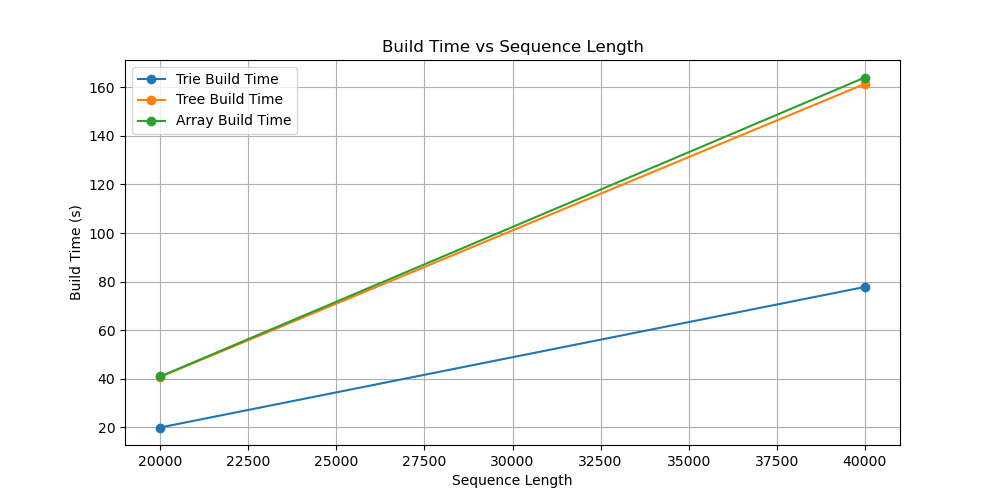
\includegraphics[width=0.6\textwidth]{build_time.png}
\caption{The average build time comparison for each indexing structure across 
different sequence lengths.}
\label{buildtime}
\end{figure}

Memory usage differs significantly between the three data structures. The 
suffix trie consumes the most memory due to its representation of 
all substrings regardless of overlap. The suffix tree reduces redundancy but 
still requires more space than the compact suffix array, which exhibits the 
lowest memory footprint (Figure~\ref{memoryusage}). This makes suffix arrays 
ideal for applications where memory is constrained.

\begin{figure}[ht] \centering
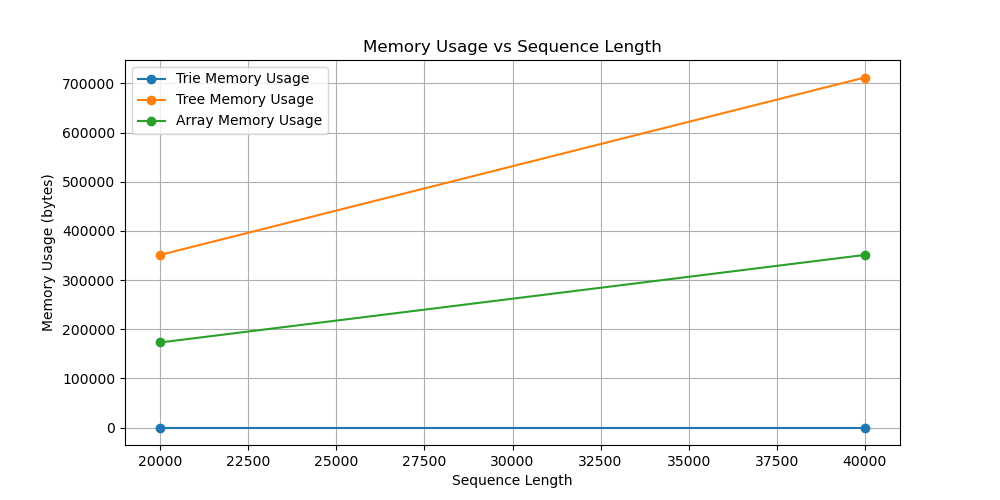
\includegraphics[width=0.6\textwidth]{memory_usage.png}
\caption{The average memory usage comparison across different sequence lengths.}
\label{memoryusage}
\end{figure}

Query performance varies across the data structures, reflecting the trade-offs 
between memory usage and speed. As shown in Figure~\ref{querytime}, suffix tries 
allow for the fastest lookups but are not memory-efficient. Suffix arrays exhibit 
the slowest query times but compensate with their minimal memory footprint. Suffix 
trees provide a middle ground, balancing query performance and memory consumption.

\begin{figure}[ht] \centering
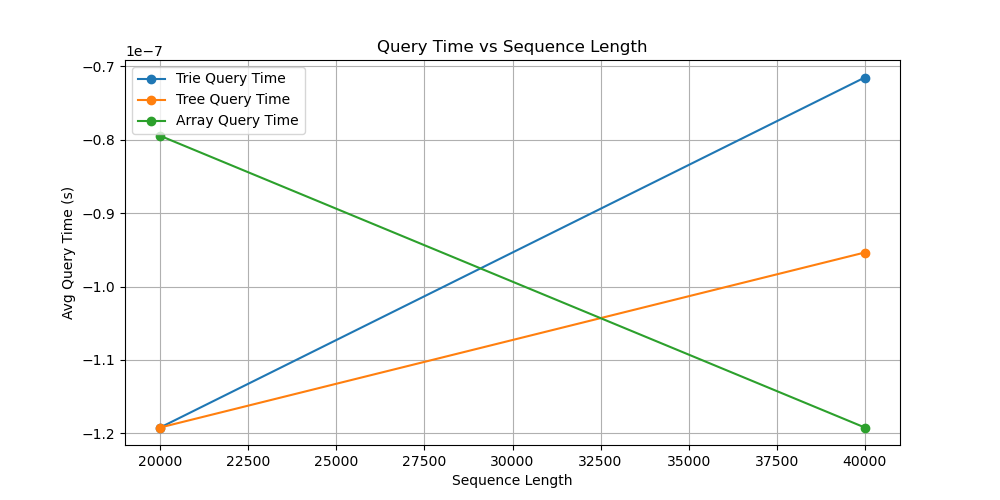
\includegraphics[width=0.6\textwidth]{query_time.png}
\caption{The average query time comparison across different sequence lengths.}
\label{querytime}
\end{figure}

\section{Methods}
To compare indexing performance, we implemented:
\begin{itemize}
\item \textbf{Suffix Trie:} A tree-based structure storing all suffixes of a string explicitly.
\item \textbf{Suffix Tree:} A compressed version of the trie, to reduce redundancy.
\item \textbf{Suffix Array:} A sorted array of suffix start positions, to allow for binary search.
\end{itemize}

We evaluated indexing performance using synthetic DNA sequences of lengths {10,000, 50,000, 100,000}
base pairs. Query substrings of lengths {5, 10, 20} were extracted from the reference sequence. For 
each structure, we measured build time, memory usage, and query time.

\subsection{Reproducibility}
To reproduce these experiments, clone the repository and execute the following command:

\begin{verbatim}
$ git clone https://github.com/cu-compg-spring-2025/assignment-6-suffix-index-audreyw04.git
$ python3 experiment.py --seq_length 10000 50000 100000 --query_length 5 10 20
\end{verbatim}

\end{document}

